
\documentclass[
	% -- opções da classe memoir --
	article,			% indica que é um artigo acadêmico
	11pt,				% tamanho da fonte
	oneside,			% para impressão apenas no verso. Oposto a twoside
	a4paper,			% tamanho do papel. 
	english,			% idioma adicional para hifenização
	brazil,				% o último idioma é o principal do documento
	]{abntex2}


% ---
% PACOTES
% ---

% ---
% Pacotes fundamentais 
% ---
\usepackage{cmap}				% Mapear caracteres especiais no PDF
\usepackage{lmodern}			% Usa a fonte Latin Modern
\usepackage[T1]{fontenc}		% Selecao de codigos de fonte.
\usepackage[utf8]{inputenc}		% Codificacao do documento (conversão automática dos acentos)
\usepackage{indentfirst}		% Indenta o primeiro parágrafo de cada seção.
\usepackage{nomencl} 			% Lista de simbolos
\usepackage{color}				% Controle das cores
\usepackage{graphicx}			% Inclusão de gráficos
\graphicspath{ {imagens/} }
\RequirePackage[onehalfspacing]{setspace}
% ---
		
% ---
% Pacotes adicionais, usados apenas no âmbito do Modelo Canônico do abnteX2
% ---
\usepackage{lipsum}				% para geração de dummy text
\usepackage{float}
\usepackage{breqn}
\restylefloat{table}
% ---
		
% ---
% Pacotes de citações
% ---
%\usepackage[brazilian,hyperpageref]{backref}	 % Paginas com as citações na bibl
\usepackage[alf]{abntex2cite}	% Citações padrão ABNT
% ---


% ---
% Informações de dados para CAPA e FOLHA DE ROSTO
% ---
\titulo{Não-linearidade na Função Reação\\ do Banco Central do Brasil}
\autor{Gustavo de Paula Ribeiro}
\local{Brasil}
\data{Junho de 2015}
% ---

% ---
% Configurações de aparência do PDF final

% alterando o aspecto da cor azul
\definecolor{blue}{RGB}{41,5,195}

% informações do PDF
\makeatletter
\hypersetup{
     	%pagebackref=true,
		pdftitle={\@title}, 
		pdfauthor={\@author},
    	pdfsubject={Tese Insper},
	    pdfcreator={Gustavo de Paula Ribeiro},
		pdfkeywords={abnt}{latex}{abntex}{abntex2}{atigo científico}, 
		colorlinks=true,       		% false: boxed links; true: colored links
    	linkcolor=blue,          	% color of internal links
    	citecolor=blue,        		% color of links to bibliography
    	filecolor=magenta,      		% color of file links
		urlcolor=blue,
		bookmarksdepth=4
}
\makeatother
% --- 

% ---
% compila o indice
% ---
\makeindex
% ---

% ---
% Altera as margens padrões
% ---
\setlrmarginsandblock{4cm}{4cm}{*}
\setulmarginsandblock{4cm}{4cm}{*}
\checkandfixthelayout
% ---

% --- 
% Espaçamentos entre linhas e parágrafos 
% --- 

% O tamanho do parágrafo é dado por:
\setlength{\parindent}{1.3cm}

% Controle do espaçamento entre um parágrafo e outro:
\setlength{\parskip}{0.2cm}  % tente também \onelineskip

% Espaçamento simples
\onehalfspacing

% ----
% Início do documento
% ----
\begin{document}

% Retira espaço extra obsoleto entre as frases.
\frenchspacing 

% ----------------------------------------------------------
% ELEMENTOS PRÉ-TEXTUAIS
% ----------------------------------------------------------

%---
%
% Se desejar escrever o artigo em duas colunas, descomente a linha abaixo
% e a linha com o texto ``FIM DE ARTIGO EM DUAS COLUNAS''.
% \twocolumn[    		% INICIO DE ARTIGO EM DUAS COLUNAS
%
%---
% página de titulo
\maketitle
\thispagestyle{empty}
\pagebreak

\begin{KeepFromToc}
  \tableofcontents
\end{KeepFromToc}
\pagebreak

% resumo em português
%\begin{resumoumacoluna}
% Conforme a ABNT NBR 6022:2003, o resumo é elemento obrigatório, constituído de
% uma sequência de frases concisas e objetivas e não de uma simples enumeração
% de tópicos, não ultrapassando 250 palavras, seguido, logo abaixo, das palavras
% representativas do conteúdo do trabalho, isto é, palavras-chave e/ou
% descritores, conforme a NBR 6028. (\ldots) As palavras-chave devem figurar logo
% abaixo do resumo, antecedidas da expressão Palavras-chave:, separadas entre si por
% ponto e finalizadas também por ponto.
 
% \vspace{\onelineskip}
 
% \noindent
% \textbf{Palavras-chaves}: latex. abntex. editoração de texto.
%\end{resumoumacoluna}

% ]  				% FIM DE ARTIGO EM DUAS COLUNAS
% ---

% ----------------------------------------------------------
% ELEMENTOS TEXTUAIS
% ----------------------------------------------------------
\textual

% ----------------------------------------------------------
% Introdução
% ----------------------------------------------------------
\section{Introdução}

	A partir do Decreto Nº 3.088, de 21 de Junho de 1999, o Brasil passou a adotar oficialmente um regime de metas para a inflação, ficando o Conselho Monetário Nacional (CMN) a cargo de fixar a meta central para a inflação e os intervalos de tolerância ao redor da mesma. O CMN também fixou como padrão para a mensuração do nível da inflação a ser adotado para o sistema de metas o Índice de Preços ao Consumidor Amplo (IPCA), mensurado e divulgado pelo Instituto Brasileiro de Geografia e Estatística (IBGE).
	
	De acordo com \citeonline{mishkin_inflation_targeting}, o regime de metas para a inflação é um arcabouço de política monetária que inclui cinco elementos: (i) o anúncio público de uma meta numérica para a inflação; (ii) um compromisso institucional com o objetivo de estabilidade de preços; (iii) a utilização de uma gama de variáveis – não só agregados monetários ou taxa de câmbio – na calibração dos instrumentos de política monetária; (iv) transparência com o público com a utilização de comunicação sobre os planos, objetivos e decisões de política e (v) responsabilização do banco central para atingir seus objetivos.
	
	\citeonline{rigolon_giambiagi}, Fischer (1995, 1996) e \citeonline{taylor_mon_pol} argumentam sobre os benefícios da adoção do Regime de Metas, quais seriam: a busca por níveis inflacionários mais baixos, dados os custos econômicos e sociais associados ao processo inflacionário, a redução de incertezas, os ganhos de eficiência alocativa e crescimento econômico, além de possibilitar a avaliação do desempenho da política monetária (comparação com o nível de inflação observado em um período com a meta adotada para o mesmo).
	
	Por conseguinte, a avaliação da dinâmica do regime de metas adotada pelo Brasil há mais de uma década se mostra tarefa pertinente. Usualmente, assume-se que o banco central reage de forma linear a desvios em relação à meta de inflação e ao produto potencial.  Porém, este pode não ser necessariamente o caso.
	
	O presente trabalho tem como objetivo testar uma possível não linearidade na função de reação do banco central e catacterizá-la, em linha com o trabalho realizado por \citeonline{pagano_rossi}, no caso brasileiro, e \citeonline{cukierman_muscatelli}, que realizaram um estudo para os Estados Unidos e Reino Unido, onde procuram por indicações de não linearidade na função de reação do banco central e o classificam como tendo preferências avessas à inflação (PAI) ou avessas à recessão (PAR).
	
	O trabalho se diferencia dos citados acima pela utilização de um método de estimação proposto por \citeonline{areosa_econometrics} que flexibiliza as hipóteses necessárias para a estimação de um modelo de regressão de transição suave, permitindo a utilização de variáveis endógenas na regressão. 
	
	Além da utilização de um método de estimação que relaxa a hipótese de exogeneidade fraca dos regressores, este trabalho também contribui para a literatura existente ao propor e utilizar uma medida alternativa de hiato do produto que é construída através da aplicação da técnica de análise de componentes principais a uma gama de séries de tempo relacionadas com o nível de atividade econômica, baseando-se nos trabalhos de \citeonline{drago_ribeiro} e da OECD (1997, 2012) na construção de indicadores de nível de atividade.
	
	\section{Revisão Bibliográfica}
	
	A partir do trabalho de \citeonline{taylor_1993}, onde sugeriu um modelo de determinação de taxa de juros a partir da taxa de inflação corrente, a taxa real de juros de equilíbrio, o hiato de inflação e o hiato do produto, vários trabalhos acadêmicos se propuseram a testar a sua validade para diferentes bancos centrais.
	
	\citeonline{judd_rudebusch} analisaram a performance de três banqueiros centrais norte-americanos, Arthur Burns, Paul Volcker e Alan Greenspan, sobre a ótica da regra de Taylor, estimando funções reação para cada período. Para Burns, encontram uma resposta fraca a desvios da inflação, sendo que a política monetária parecia responder mais fortemente ao ciclo do produto. Volcker, por sua vez, parece ter adotado uma função reação que respondia fortemente à inflação. 
	
	Já o banco central comandado por Greenspan parecia responder ao hiato do produto de forma mais agressiva do que a assumida inicialmente por \citeonline{taylor_1993}. Concluem que o arcabouço apresentado por \citeonline{taylor_1993} se mostrou útil para analisar elementos chave da política monetária implementada por cada banqueiro central.
	
	No caso europeu, \citeonline{gerlach} analisaram os movimentos de taxas de juros nos países que iriam à época fazer parte da Zona do Euro. Demostraram que, ao agregar as respostas dos bancos centrais de cada país, a função de reação encontrada seguia uma relação como a sugerida pela regra de Taylor.
	
	\citeonline{ullrich} analisou se o banco central americano, o \textit{Federal Reserve} (Fed), e se o banco central europeu (ECB) utilizam políticas que podem ser descritas a partir da regra proposta por \citeonline{taylor_1993}. Para o período anterior a 1999, início da união monetária na Zona do Euro, a resposta média de política monetária dos países que passaram a compor a Zona do Euro parecia incorporar uma forte reação à inflação, com coeficiente de longo prazo estimado que excede o valor unitário, em linha com os achados de \citeonline{gerlach}. Porém, após 1999, o coeficiente estimado se mostra como menor que um. Já o Fed mostrou respostas em linha com a regra de Taylor proposta a partir de 1999, porém o estudo é inconclusive para o período de 1995 a 1998.
	
	Já \citeonline{surico} investigou a possibilidade do Fed adotar pesos diferentes para desvios positivos ou negativos a desvios da inflação à meta ou de hiatos do produto positivos ou negativos. Encontrou evidências de que, no período anterior a 1979, o Fed parecia incorporar uma resposta maior a hiatos do produto em campo negativo, o que gerou um viés inflacionário médio da ordem de 1,5\%. Com o início da era Volcker, no entanto, este viés inflacionário deixou de existir, com o Fed adotando respostas simétricas aos desvios do hiato do produto e da inflação. Os autores argumentam que este fato contribuiu para uma porção significativa da desinflação observada no período.
	
	Para o caso brasileiro, \citeonline{mendonca} estruturou uma regra de Taylor linear onde assume pesos iguais ao hiato do produto e da inflação, incluindo também a taxa de juros americana para capturar a conjuntura macroeconômica externa, preocupando-se também com o resultado da determinação de juros no Balanço de Pagamentos. Chega à conclusão que o banco central brasileiro não segue a regra de Taylor prosposta.
	
	\citeonline{areosa_target} derivam uma curva de Phillips Novo Keynesiana incorporando, além da indexação à inflação passada, a própria meta de inflação, encontrando que o parâmetro associado à meta é estatisticamente significante.
	
	\citeonline{bevilaqua} coletam evidências de que a existência de metas de inflação contribuiu para o aperfeiçoamento do ambiente macroeconômico no Brasil, criando um ambiente mais estável e previsível. Apontam como argumento a favor disto o fato de, após a parada abrupta de influxos de capital e a forte depreciação da moeda brasileira em 2002, os erros de previsão da inflação 12 meses a frente em comparação com a inflação observada caíram, indicando que, após um período inflacionário, a reversão da aceleração de preços contribuiu para a formação de expectativas ancoradas.
	
	Buscando possíveis assimetrias nos objetivos do banco central brasileiro, \citeonline{aragon_portugal} encontraram, para o período amostral de 2000 a 2007, evidências de que o Banco Central do Brasil foi mais avesso a desvios negativos da inflação à meta. Porém, reconhecem que este resultado pode ter sido influenciado por decisões de política tomadas em momentos de crise, como em 2001 e 2002, e focaram então o estudo ao período de 2004 a 2007, não encontrando evidências de assimetrias na função reação do banco central.
	
	Por fim, \citeonline{pagano_rossi} utilizaram o arcabouço apresentado por \citeonline{cukierman_muscatelli}, onde classificam um banco central entre tendo preferências avessas à inflação, quando reagem mais fortemente a hiatos da inflação positivos, ou avessas à recessão, com reações mais relevantes a hiatos do produto negativos. Seus resultados rejeitam a hipótese de linearidade na função reação do banco central, além de indicar preferências de aversão à recessão (PAR).
	
	\citeonline{cukierman_muscatelli} elaboram quatro possibilidades de preferências do banco central:
	
	\begin{enumerate}
		\item Caso o banco central tenha preferências de aversão à recessão (PAR), mas não à inflação (PAI), a função reação é côncava tanto no hiato da inflação quanto no do produto;
		\item Ao contrário, caso o banco central apresente PAI mas não PAR, a função reação é convexa em ambos;
		\item Caso o banco central seja tanto PAI quanto PAR, a função de reação é linear caso os efeitos sejam de magnitude semelhante, ou côncava ou convexa dependendo do efeito dominante;
		\item A função de reação é linear, não havendo nem PAI nem PAR.
	\end{enumerate}
	
	\section{Modelo Teórico}
	
	Segundo \citeonline{cukierman_muscatelli}, o objetivo da autoridade monetária pode ser entendido como o de minimizar a função:
	
	\begin{equation}  \label{funcao_perda}
		E_0\sum_{t=0}^{\infty}\delta^t L_t
	\end{equation}
	%
	onde $\delta$ é o fator de desconto e $L_{t}$ representa a função perda do banco central, dada pela equação:
	
	\begin{equation}
		L_t = Af(x_t) + h(\pi_t - \pi^*),
	\end{equation}
	%
	onde $x_t$ é o hiato do produto, $\pi_t$ a inflação corrente e $\pi_t^*$ a meta de inflação vigente. As funções $f$ e $h$ possuem as seguintes propriedades:
	
	\begin{eqnarray}
		f'(x_t) < 0 \mbox{ para } x_t < 0 \mbox{, } f'(y_t) \geq 0 \mbox{ para } x_t \geq 0 \mbox{, } f(0) = f'(0) = 0,\nonumber \\
		f''(x_t)>0 \mbox{, } f'''(x_t) \leq 0,\nonumber \\
		h'(\pi_t-\pi^*) \leq 0 \mbox{ para } \pi_t - \pi^* \leq 0, \nonumber \\
		h'(\pi_t-\pi^*) > 0 \mbox{ para } \pi_t - \pi^* > 0, \nonumber \\
		h(0)=h'(0)=0 \mbox{, } h''(\pi_t-\pi^*)>0 \mbox{, } h'''(\pi_t-\pi^*) \geq 0
	\end{eqnarray}
	%
	de onde tem-se que as perdas advindas do hiato do produto e dos desvios da inflação em torno da meta atingem seus valores mínimos quando ambos desvios são zero. Ao mesmo tempo, quanto maior o hiato do produto ou os desvios da inflação em termos absolutos, maiores são as perdas associadas. 
	
	Assim como em uma função quadrática de perda do banco central, as derivadas parciais de segunda ordem são assumidas como zero, porém, diferentemente do caso quadrático, elas não necessariamente são simétricas em torno de zero, podendo as derivadas parciais de terceira ordem assumirem valores diferentes de zero.
	
	A estrutura econômica assumida no modelo se dá por um arcabouço Novo Keynesiano linear de preços rígidos, conforme exposto por \citeonline{clarida_mon_policy}, porém também utilizando o hiato do produto e a inflação defasados em um período, para abranger possíveis efeitos inerciais.
		
	\begin{equation}  \label{curva_is}
		x_t=-\varphi(i_t-E_t\pi_{t+1}) + E_tx_{t+1} + \eta x_{t-1} + u_t
	\end{equation}
	
	\begin{equation} \label{curva_phillips}
		\pi_t = \lambda x_t + bE_t\pi_{t+1} + \omega \pi_{t-1} + g_t
	\end{equation}
%
	onde $E_tx_{t+1}$ e $E_t\pi_{t+1}$ representam os valores esperados do hiato do produto e da inflação condicionados às informações disponíveis até $t$. $i_t$ é a taxa nominal de juros, $g_t$ e $u_t$ são inovações independentes assumidas como processos ruídos brancos representando choques de oferta e de demanda, respectivamente. 
	
	Os parâmetros $\varphi$, $\lambda$ e $b$ são todos positivos. Ou seja, a inflação corrente depende das expectativas sobre a inflação futura e do hiato do produto, enquanto o hiato do produto depende da taxa real de juros e da expectativa sobre o hiato futuro do produto.
	
	Assim, de acordo com \citeonline{cukierman_muscatelli}, a análise sobre a aversão do banqueiro central à recessão ou à inflação se dá através da terceira derivada das funções $f$ e $h$ dentro da função perda do banco central. 
	
	Uma terceira derivada negativa na função $f$ representa maior aversão a hiatos negativos do produto do que a hiatos positivos pois, no caso de uma terceira derivada negativa de $f$, quanto mais positivamente o hiato do produto se torna, menor é a perda marginal por estar distante do hiato neutro de produto. Analogamente, uma terceira derivada positiva na função $h$ representa um banqueiro central mais avesso a níveis de inflação acima da meta do que o contrário.	
	
	Para verificar tais afirmações, uma análise gráfica pode se mostrar útil. Tomando como exemplo as seguintes formais funcionais para $f$ e $h$:
	
	\begin{equation}
		f(x_t) = \frac{(e^{\gamma x_t} - \gamma x_t - 1)}{\gamma^2} 
	\end{equation}
	
	\begin{equation}	
		h(\pi_t - \pi^*) = \frac{(e^{\alpha (\pi_t - \pi^*)} - \alpha (\pi_t - \pi^*) - 1)}{\alpha^2}
	\end{equation}
%
	tem-se que a função perda do banco central assume a seguinte caracterização, tal como proposto no trabalho realizado por \citeonline{aragon_portugal}:
	
	\begin{equation} \label{eq_aragon_portugal}
		L_t = A \frac{(e^{\gamma x_t} - \gamma x_t - 1)}{\gamma^2} + \frac{(e^{\alpha (\pi_t - \pi^*)} - \alpha (\pi_t - \pi^*) - 1)}{\alpha^2}
	\end{equation}
	
	As derivadas terceiras de $f$ e de $h$ com função a $x_t$ e $(\pi_t - \pi^*)$, por sua vez, são dadas, respectivamente, por:
	
	\begin{equation}
		\frac{df^3}{dx_t^3} = \gamma e^{\gamma x_t}
	\end{equation}
	
	\begin{equation}
		\frac{dh^3}{d(\pi_t - \pi^*)_t^3} = \alpha e^{\alpha (\pi_t - \pi^*)}
	\end{equation}
	
	É importante notar que para valores de $\gamma$ e $\alpha$ diferentes de zero, as terceiras derivadas acima também são diferentes de zero, introduzindo assimetrias na função perda do banco central. Assumindo, por exemplo, $\gamma = -1.0$ e $\alpha = 1.0$, tem-se que a terceira derivada de $f$ é negativa em relação ao hiato do produto, enquanto a terceira derivada de $h$ é positiva em relação aos desvios da inflação à meta.
	
	Assim, ao analisar graficamente a função perda dada por (\ref{eq_aragon_portugal}), com os valores de $\gamma$ e $\alpha$ assumidos acima, tem-se que a perda relacionada a um hiato do produto negativo é maior do que a relacionada ao mesmo hiato do produto positivo, enquanto a perda relacionada a desvios positivos da inflação à meta é maior que a desvios negativos da inflação à meta, para cada desvio absoluto.
		
			
	%\begin{figure}
  %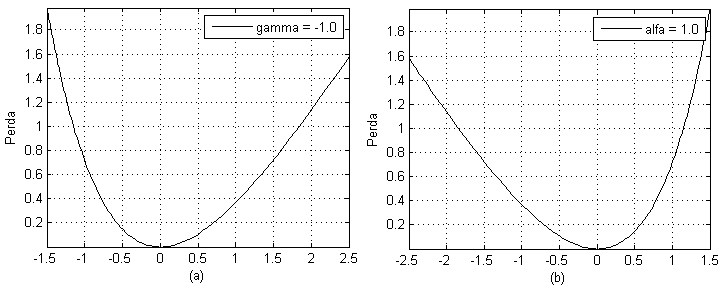
\includegraphics[height=2cm,keepaspectratio,left]{D:/Documents/Dissertacao/imagens/funcao_perda_assimetrica.png}
	%\caption{Função de reação do banco central assimétrica ao hiato do produto e a desvios da inflação em torno da meta}
	%\end{figure}
	
	\begin{figure}
	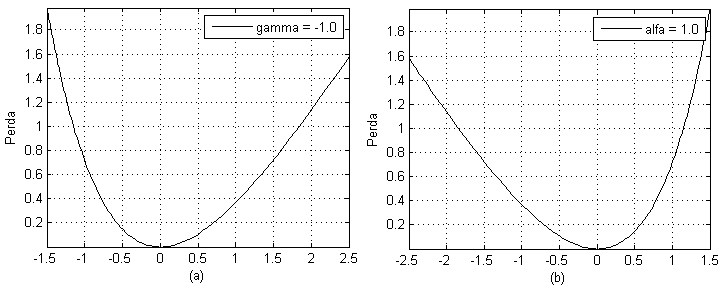
\includegraphics[scale=0.7]{D:/Documents/Dissertacao/imagens/funcao_perda_assimetrica.png}
	\caption{Função de reação do banco central assimétrica ao hiato do produto $(a)$ e a desvios da inflação em torno da meta $(b)$}
	\label{fig:funcao reacao assimetrica}
	\end{figure}
	

	
	Para o restante do presente trabalho, não serão assumidas formais funcionais explícitas para $f$ e $h$. A regra de política monetária, por fim, é encontrada na minimização da equação (\ref{funcao_perda}) sujeita às restrições presentes em (\ref{curva_is}) e (\ref{curva_phillips}). Substituindo (\ref{curva_is}) e (\ref{curva_phillips}) em (\ref{funcao_perda}), temos:
	
	\begin{eqnarray}
		E_0\sum_{t=0}^{\infty}\delta^t \{ Af(-\varphi(i_t-E_t\pi_{t+1}) + E_tx_{t+1} + \eta x_{t-1} + u_t) +\nonumber \\ \lambda x_t + bE_t\pi_{t+1} + \omega \pi_{t-1} + g_t \}
		%E_0\sum_{t=0}^{\infty}\delta^t\{Af[-\varphi(i_t - E_t\pi_{t+1}) + E_tx_{t+1} + g_t] +\nonumber \\ h[\lambda(-\varphi(i_t-E_t\pi_{t+1}) + E_tx_{t+1} + g_t) + bE_t\pi_{t+1} + u_t - \pi^*]\}
	\end{eqnarray}
	
	Ainda de acordo com \citeonline{cukierman_muscatelli}, os formuladores de política monetária, sob discricionariedade, reotimizam o problema a cada período tomando as expectativas futuras das variáveis como dadas. A condição de primeira ordem é dada por:
	
	\begin{equation}
		AE_tf^'[.] + \lambdaE_th^'[.] = 0, t = 0, 1, 2, ...,
	\end{equation}

	Com isto, a taxa de juros é escolhida como função dos hiatos de inflação e produto esperados para o período seguinte.
	
	Como as formas funcionais de $f(.)$ e $h(.)$ não são explicitadas, não é possível resolver explicitamente a minimização da função de perda do banco central, como seria no caso de uma função quadrática. Diante disto, podemos apenas inferir algumas características da função de reação do mesmo e as relações com os dois tipos de assimetrias estudadas para as preferências do banqueiro central utilizando estatísticas comparativas. Diferenciando a condição de primeira ordem em $t=0$ para $E_0\pi_1$, temos:
	
	\begin{equation}
		\frac{di_0}{dE_0\pi_1} = \frac{1}{\varphi} \frac{\varphiAE_0f_0^{''}[.] + \lambda(\varphi\lambda + b)E_0h_0^{''}[.]}{AE_0f_0^{''}[.] + \lambda^2E_0h_0^{''}[x]} \equiv \frac{\varphiAE_0f_0^{''}[.] + \lambda(\varphi\lambda + b)E_0h_0^{''}[.]}{\varphi D}
	\end{equation}
	
	É importante notar dois pontos: (1), a derivada acima é positiva, o que implica que o banco central reaje a aumentos da inflação esperada aumentando a taxa de juros e (2) o numerador é maior que o denominador, implicando que o aumento na taxa de juros real é maior do que o aumento nas expectativas de inflação.
	
	Ao realizar a derivada acima em relação a $E_0x_1$, temos:
	
	\begin{equation}
		\frac{di_0}{dE_0\x_1} = \frac{1}{\varphi} \frac{A(1+\varphi\lambdaE_0f_0^{''}[.] + \lambda^2(1 + \varphi\lambda + b)E_0h_0^{''}[.]}{D} 
	\end{equation}
	
	Resultado também positivo, implicando que a taxa de juros se eleva em resposta a um aumento nas expectativas do hiato do produto.
	
	Conforme visto, caso o banco central não apresente nem PAR e nem PAI, sua função de reação é linear, sendo que a função de perda é quadrática tanto na inflação quanto no hiato do produto. Assim, como \textit{benchmark}, será utilizada a seguinte função de reação para o banco central, generalizada a partir de \citeonline{taylor_1993} por \citeonline{pagano_rossi}, que relaciona linearmente a taxa de juros aos hiatos da inflação e produto:
	
	\begin{equation}
		i_t^* = \bar{i} + \beta E_t(\pi_{t+k} - \pi^*) + \Phi x_{t-j}
	\end{equation}
	
	Aqui, $E_t(\pi_{t+k} - \pi^*)$ representa o desvio esperado da inflação em relação à meta $k$ períodos à frente, $x_{t-j}$ representa o hiato do produto com $j$ defasagens e $\bar{i}$ é a taxa de juros nominal vigente. Para observar a possibilidade de suavização dos movimentos de taxa de juros, é adotado um mecanismo de ajuste parcial, conforme \citeonline{cukierman_smooth}:
		
	\begin{equation}
		i_t = \rho i_{t-1} + (1-\rho) i_t^*
	\end{equation}
	%
	onde $\rho$ é um coeficiente que indica o grau de suavização do banqueiro central com relação a movimentos na taxa de juros. Utilizando este parâmetro de suavização na função de reação adotada, temos:
	
	\begin{equation}
		i_t = \rho i_{t-1} + (1-\rho) \{ \bar{i} + \beta E_t(\pi_{t+k} - \pi^*) + \Phi x_{t-j} \}
	\end{equation}
	
	A ser estimada por Mínimos Quadrados Ordinários.
	
	Por fim, para modelar a resposta não linear do banqueiro central, um modelo STR (\it{Smooth Transition Regression) é utilizado para a função de reação do banco central, incorporando funções de transição para o hiato do produto e desvios da inflação. Para tanto, estas funções são adicionadas à forma linear anteriormente exposta como variáveis de transição:
	
	\begin{equation}
		i_t^* = X_t \Beta + X_t \alpha_\pi \theta(\Gamma,c,z_{t-d}^\pi) + X_t \alpha_x \theta (\Gamma,c,z_{t-j}^x+e_t)
	\end{equation}
	%
	onde $X_t$ representa as variáveis do modelo linear, $z_{t-d}^\pi$ e $z_{t-j}^x$ são as variáveis de transição referentes ao hiato do produto e o desvio da inflação, $c$ é o limiar a partir do qual ocorre a mudança de regime, $\Gamma$ é o parâmetro de suavização da transição, $\theta(.)$ é uma função logística, escolhida segundo o trabalho de \citeonline{areosa_econometrics} e os resultados obtidos por \citeonline{pagano_rossi}. Com as devidas restrições aos vetores de parâmetros $\alpha_\pi$ e $\alpha_x$, a função de reação é dada por:
	
	\begin{equation}
		i_t^* = \bar{i} + \beta E_t(\pi_{t+k} - \pi^*) + \Phi x_{t-f} + \alpha_\pi E(\pi_t - \pi^*)\theta(H_{t-d}^\pi) + \alpha_x x_{t-f} \theta (H_{t-j}^x) + u_t
	\end{equation}
	
	Seguindo o procedimento adotado no modelo não linear, utilizamos aqui também um termo de suavização dos movimentos da taxa de juros, chegando no seguinte formato para a função de reação:
	
	\begin{eqnarray}  \label{modelo_nao_linear}
		i_t = \rho i_{t-1} + (1-\rho) \{ \bar{i} + \beta E_t(\pi_{t+k} - \pi^*) + \Phi x_{t-f} + \nonumber \\ 
		 \alpha_\pi E(\pi_t - \pi^*)\theta(H_{t-d}^\pi) + \alpha_x x_{t-f} \theta (H_{t-j}^x) + u_t \}
	\end{eqnarray}
	
	\section{Extensão dos trabalhos existentes}	
	
	Modelos STR são largamente utilizados para capturar comportamentos assimétricos de séries de tempo. Sobre a hipótese de exogeneidade, o método de estimação usualmente utilizado é o de Mínimos Quadrados Não Lineares. \citeonline{cukierman_muscatelli} e, por conseguinte, \citeonline{pagano_rossi} assumiram a exogeneidade das variáveis utilizadas na função reação do banco central e utilizaram Mínimos Quadrados para estimar os parâmetros do modelo STR estudado, porém, na hipótese de que o hiato do produto e os desvios da inflação à meta são endógenos, tal estimação torna-se viesada.
	
	\citeonline{areosa_econometrics} relaxam a suposição de exogeneidade fraca ao propor um estimador GMM para recuperar os parâmetros dos modelos STR.	Utilizando este método de estimação para a equação \ref{modelo_nao_linear}, não mais será necessária a hipótese de exogeneidade das variáveis de hiato do produto e desvios da inflação, mantendo não viesados as estimações dos parâmetros mesmo na presença de endogeneidade destas variáveis.
	
	Além do mais, \citeonline{pagano_rossi} utilizaram, como medida do hiato do produto, o componente cíclico da produção industrial brasileira, tal qual é divulgada pelo IBGE. Neste trabalho, propomos a utilização de uma medida de hiato de produto mais ampla, baseada no IBC-Br, \textsl{proxy} de PIB mensal computado pelo Banco Central do Brasil que leva em consideração a produção industrial, as vendas no varejo e a produção agropecuária. Como não necessariamente o banqueiro central tem disponível o último dado referente a esta série em tempo real para a tomada de decisão de política monetária, propomos uma estimação do hiato do IBC-Br a partir da utilização de análise de componentes principais.
	
	
	\section{Dados Utilizados}
	Os dados utilizados têm início em janeiro de 2003 (início da série do IBC-Br) e fim em dezembro de 2014, com periodicidade mensal. Durante todo este período, o Brasil esteve sob regime de câmbio flutuante e de metas de inflação. Como medida de inflação, será utilizada a expectativa 12 meses à frente suavizada das projeções FOCUS, pesquisa realizada pelo Banco Central do Brasil com participantes do mercado, do primeiro dia útil de cada mês. O instrumento de política monetária a ser utilizado é a meta para a taxa Selic, definida pelo Banco Central.
	
	Como medida de hiato do produto, é proposta neste trabalho a utilização de uma medida alternativa através de um indicador através da utilização de análise de componentes principais a uma gama de variáveis coincidentes de atividade. Isto é feito por dois motivos: extrair a tendência comum desta série de indicadores e conseguir uma medida quase em tempo real do nível de atividade.
	
	A utilização desta medida alternativa se dá como maneira de projetar em um determinado instante do tempo as condições atuais da economia, resumidas pelo indicador mensal do Banco Central do Brasil chamado de IBC-Br. Como no momento da decisão de política monetária as últimas informações referentes a este indicador não necessariamente são conhecidas, aplicaremos a metodologia aqui descrita para projetá-lo em cada instante de tempo.
	
	A OCDE (2012) propõe retirar a tendência e suavizar os indicadores utilizados para compor seus indicadores de nível de atividade através do uso do filtro Hodrick-Prescott, dada a sua maior estabilidade e transparência quando comparado com outros filtros estatísticos\footnote{A OCDE (2012) testa a utilização, além do filtro HP, do Phase Average Trend Method (PAT), do Month for Cyclical Dominance method (MCD) e do Christiano-Fitzgerald Filter (CF), acabando por concluir pela utilização do filtro HP.}.
	
	Após a extração dos componentes cíclicos das variáveis candidatas, a análise de componente principal é utilizada e os componentes resultantes que explicam a maior parte da variabilidade dos dados originais são regredidos contra o ciclo do IBC-Br até $t_-1$, para termos então a projeção deste indicador em $t_0$.
	
	Para isto, e de acordo com os trabalhos de \citeonline{drago_ribeiro} e da OCDE (1997 e 2012), a modelagem aqui proposta se dá pelos seguintes passos:
	
	\begin{enumerate}
		\item Dessazonalização das séries dos indicadores escolhidos;
		\item extração de uma tendência de longo prazo com a utilização de um filtro HP com parâmetro de 14.400;
		\item aplicação de um filtro HP com parâmetro 10 ao componente cíclico;
		\item extração do componente cíclico do IBC-Br através da mesma metodologia explicitada acima;
		\item construção da medida de hiato pela regressão dos componentes principais que explicam pelo menos 85\% da variabilidade total dos dados com o componente cíclico do IBC-Br.
	\end{enumerate}
	
	Como variáveis candidatas, foram escolhidas séries de tempo com divulgação rápida, geralmente conhecidas antes da divulgação da produção industrial de determinado mês. A relação completa das séries utilizadas se encontra no Apêndice A.
	
	%Abaixo, o resultado da metodologia descrita acima, resultando na medida de hiato do produto a ser utilizada neste trabalho:
		
		
	%\begin{figure}[b]
	%	\begin{center}
	%	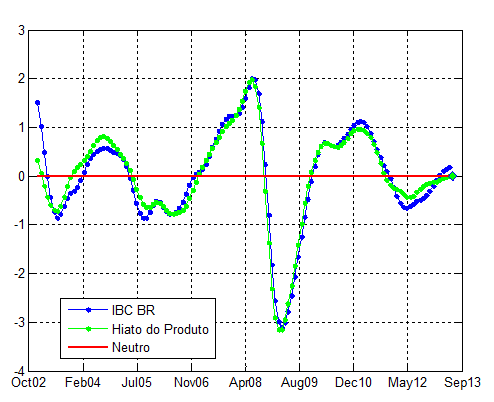
\includegraphics[scale=0.65]{D:/Documents/Dissertacao/imagens/hiatos.PNG}
	%	\captionof{Comparação de Hiatos: IBC-Br vs Medida Proposta}
	%	\end{center}
	%\end{figure}
		
	
	\section{Resultados Esperados}
	
	Na conclusão deste trabalho de pesquisa, espera-se implementar o método de estimação proposto por \citeonline{areosa_target} e utilizá-lo no modelo teórico aqui apresentado. Com isto, espera-se podermos concluir sobre as preferências do Banco Central do Brasil sem precisar utilizarmos da hipótese de exogeneidade das variáveis utilizadas, principal crítica que temos aos trabalhos anteriores que seguiram esta linha de pesquisa.

	\newpage

\bibliography{disc}

%	\section{Bibliografia}
	

	
%	ALVES, Sergio e Waldyr, AREOSA, 2005. \textbf{Targets and Inflation Dynamics}. Texto para Discussão n. 100, Banco Central do Brasil.
	
%	ARAGÓN, Edilean K. S. B., PORTUGAL, M. S., 2010. \textbf{Nonlinearities in Central Bank of Brazil's reaction function: the case of asymmetric preferences}. Estudos Econômicos (São Paulo), vol.40, n.2.
	
%	AREOSA, Waldyr Dutra, MCALEER, Michael e MEDEIROS, Marcelo C., 2011.\textbf{Moment-based estimation of smooth transition regression models with endogenous variables}.  Journal of Econometrics, Elsevier, vol. 165(1), pg 100-111.
	
%	BEVILAQUA, Afonso, MESQUITA, Mário e MINELLA, André, 2007. \textbf{Transmission Mechanisms for Monetary Policy in Emerging Market Economies}.  Bank for International Settlements, Paper n. 35.
	
%	BRASIL, Decreto nº 3.088 de 21 de Junho de 1999. \textbf{Estabelece a sistemática de "metas para a inflação" como diretriz para fixação do regime de política monetária e dá outras providências}. Presidência da República.
	
%	CLARIDA, Richard, et al, 1998.\textbf{Monetary Policy Rules in Practice: Some International Evidence}. European Economic Review, v42, pg. 1033-1067.
	
%	CUKIERMAN, Alex 1990. \textbf{Why Does the Fed Smooth Interest Rates}. Monetary Policy on the Fed's 75th Anniversary. Proceedings of the 14th Annual Economic Policy Conference of the Federal Reserve Bank of St. Louis. 1990. Kluwer Academic Publishers, pp. 111-147.
	
%	CUKIERMAN, Alex e MUSCATELLI, Anton, 2008. \textbf{Nonlinear Taylor Rules and Asymmetric Preferences in Central Banking: Evidence from the United Kingdom and the United States}. The B.E. Journal of Macroeconomics, Vol. 8(1), Artigo 7.
	
%	DRAGO, Alessandro e RIBEIRO, Gustavo, 2013. \textbf{Indicadores para Projeção do Nível de Atividade Econômica no Brasil}. Seminário sobre Crescimento Econômico, março de 2013, Brasília: Ministério da Fazenda e Banco Interamericano de Desenvolvimento
	
%	FISCHER, Stanley, 1996.\textbf{ Why are Central Banks Pursuing Long-Run Price Stability?}. Simpósio do Federal Reserve Bank de Kansas City, Achieving Price Stability.
	
%	______, 1995.\textbf{ Modern Approaches to Central Banking}. National Bureau of Economic Research, Working Paper 5064. Cambridge, MA.
	
	%JUDD, P. e RUDEBUSCH, G, 1998. \textbf{Taylor’s Rule and the Fed: 1970 – 1997}. Federal Reserve Bank of San Francisco Economic Review, n3, pg. 16.
	
%	MENDONÇA, Helder Ferreira, 2001. \textbf{Mecanismos de transmissão monetária e a determinação da taxa de juros: uma aplicação da regra de Taylor ao caso brasileiro}. Economia e Sociedade, v 15, pg. 65-81.
	
%	MISHKIN, Frederic, 2000.\textbf{ Inflation Targeting in Emerging Market Countries}. American Economic Review, American Economic Association, vol. 90(2), pg. 105-109.

%	OECD, 2012. \textbf{OECD System of Composite Leading Indicators}. Short-term Economic Statistics Division, Statistics Directorate.
	
%	OECD, 1997. \textbf{Cyclical Indicators and Business Tendency surveys}. OECD/GD(97)58, General Distribution.
	
%	PAGANO, Terence de A. e ROSSI, José Luiz J., 2009. \textbf{Uma análise da não-linearidade da função de reação do Banco Central do Brasil: Avesso a Inflação ou a Recessão?}. Ibmec Working Papers wpe_188, Insper Working Paper, Insper Instituto de Ensino e Pesquisa.
	
%	RIGOLON, Francisco e GIAMBIAGI, Fabio, 1999. \textbf{A atuação do Banco Central em uma economia estabilizada: é desejável adotar metas inflacionárias no Brasil?}. Revista de Economia Política 19(3), pg. 3-22
	
%	TAYLOR, John, 1993. \textbf{Discretion versus policy rules in practice}. Carnegie-Rochester Conference Series on Public Policy, vol. 39, pg. 195-214

%  ______, 1996.\textbf{Policy rules as a means to a more effective monetary policy}. BOJ Monetary and Economic Studies, vol. 14, n. 1.

\pagebreak

\begin{appendices}
\chapter{Variáveis candidatas}

	
\begin{table}[H]
		\centering
			\begin{tabular}{lll}
			\hline
			Variável & Fonte \\ \hline
			NUCI & FGV \\
			Confiança da Indústria & FGV \\
			Confiança do Comércio & FECOMERCIO \\
			Confiança do Comércio & FECOMERCIO \\
			Índice de Atividade no Comércio & Serasa Experian \\
			Subíndice de Venda de Veículos & Serasa Experian \\
			Subíndice de Venda em Supermercados & Serasa Experian \\
			Subíndice de Venda de Eletrodomésticos & Serasa Experian \\
			Subíndice de Venda de Combustíveis & Serasa Experian \\
			Subíndice de Venda de Itens de Vestuário & Serasa Experian \\
			Subíndice de Venda de Materiais de Construção & Serasa Experian \\
			Produção Total de Veículos & ANFAVEA \\
			Demanda de Energia Elétrica & ONS \\
			Fluxo de Veículos Pesados em Estradas Pedagiadas & ABCR \\
			Emplacamento Total de Veículos & FENABRAVE \\
			Emplacamento de Veículos Comerciais Leves & FENABRAVE \\
			Emplacamento de Caminhões & FENABRAVE \\
			Emplacamento de Ônibus & FENABRAVE \\
			Emplacamento de Motocicletas & FENABRAVE \\
			Índice de Commodities Total & CRB - \textsl{Commodity Research Bureau} \\
			Índice de Commodities - Fat & CRB - \textsl{Commodity Research Bureau} \\
			Índice de Commodities - Food & CRB - \textsl{Commodity Research Bureau} \\
			Índice de Commodities - Live Stock & CRB - \textsl{Commodity Research Bureau} \\
			Índice de Commodities - Metals & CRB - \textsl{Commodity Research Bureau} \\
			Índice de Commodities - Raw Industrials & CRB - \textsl{Commodity Research Bureau} \\
			Índice de Commodities - ISM Manufacturing & \textsl{Institute for Supply Management} \\
			Taxa de Câmbio Reais por Dólar & Banco Central do Brasil \\ \hline
			\end{tabular}
		\caption{Variáveis Candidatas}
		\label{tab:VariáveisCandidatas}
	\end{table}	
	
\end{appendices}

\end{document}
